\documentclass[compress]{beamer}
%for printing or having a crappy pdf reader backup
%\documentclass[handout]{beamer}
\mode<presentation>
\usetheme{Madrid}


\usecolortheme[RGB={128,128,128}]{structure}
\definecolor{my_gray}{RGB}{105,105,105}
\setbeamercolor{khumna}{fg=white,bg=my_gray}
%teal \usecolortheme[RGB={0,128,128}]{structure}
%\useoutertheme{miniframes}
\useinnertheme{default}
\usepackage{color}
\definecolor{Maroon}{RGB}{80,0,0}
\definecolor{BurntOrange}{RGB}{204,85,0}
\usepackage{setspace}
\usepackage{amsmath}
\usepackage{amsthm}
\usepackage{amsfonts}
\usepackage{amssymb}
\usepackage{verbatim}
\usepackage{array}
\usepackage{graphicx}
\usepackage{subfigure}
\usepackage{colortbl}
%\usepackage[retainorgcmds]{IEEEtrantools}
\usepackage{wrapfig}
\usepackage[figurename=,tablename=]{caption}
\usepackage{multirow}
\setbeamercolor{normal text}{fg=black}
\setbeamercovered{dynamic}
\beamertemplatetransparentcovereddynamicmedium
%\usepackage{chronology}
\setbeamertemplate{caption}[numbered]
\usepackage{colortbl}
\newcommand {\mathsym}[1]{{}}
\newcommand {\unicode}{{}}
\newcommand{\om}{\boldsymbol{\Omega}}
\newcommand{\etal}{{\it et al.\,}}
\newcommand{\vr}{\vec{r}}
\newcommand{\vo}{\vec{\Omega}}
\newcolumntype{L}{>{\centering\arraybackslash}m{3cm}}
\newcommand{\tcr}[1]{\textcolor{red}{#1}}
%Creating a norm command
\newcommand{\norm}[1]{\left\lVert#1\right\rVert}
%Allow page breaks within align
\allowdisplaybreaks
%Putting logo and banner in title and adding banner
\usepackage{textpos}
%Importing csv's directly
\usepackage{pgfplotstable}
%Code
\usepackage{listings}
\usepackage{epstopdf}
\usepackage{pdfpages}
\newlength \figwidth
\setlength \figwidth {0.5\textwidth}

\newcommand{\backupbegin}{
   \newcounter{finalframe}
   \setcounter{finalframe}{\value{framenumber}}
}
\newcommand{\backupend}{
   \setcounter{framenumber}{\value{finalframe}}
}

\addtobeamertemplate{frametitle}{}
{
	\begin{textblock*}{100mm}(0.85\textwidth,-1cm)
	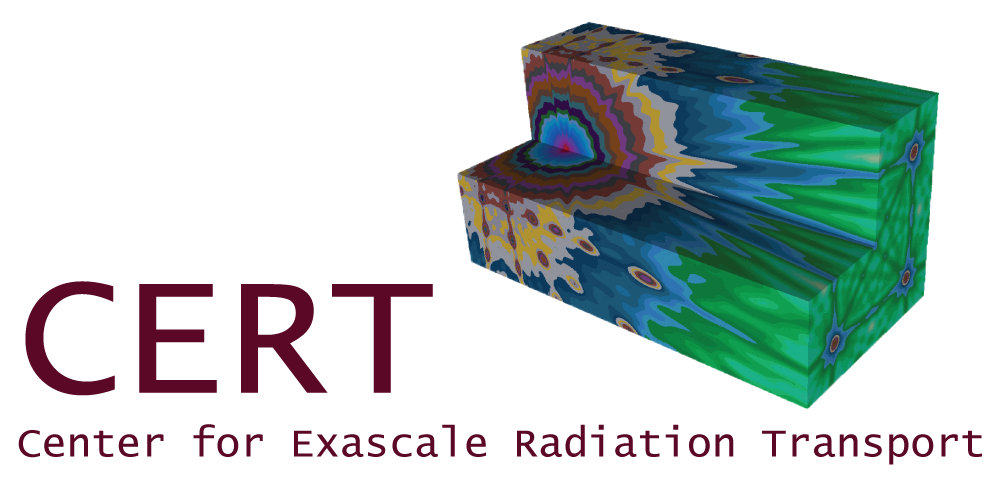
\includegraphics[height = 1cm,width=2cm]{figures/cert_logo_maroon.png}
	\end{textblock*}
}
\beamertemplatenavigationsymbolsempty



\begin{document}
%	

\title[Load Balancing]{An Update to Mesh Generation and Load Balancing in PDT}
\author[Ghaddar]{Tarek Ghaddar \\  Dr. Jean Ragusa}
\institute[TAMU]{Texas A\&M University}
%\committee{Morel,Popov}{Dr. Jim Morel \\ Dr. Bojan Popov}
\date[April 5, 2016]

{
\setbeamertemplate{headline}{}
\begin{frame}
\vspace{-1.1cm}
	\begin{figure}[t]
		\centering
			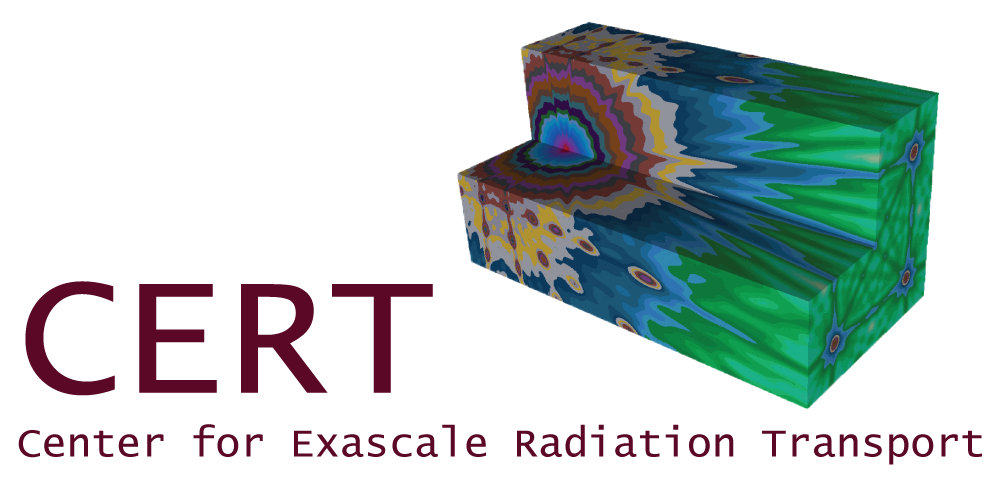
\includegraphics[width=.25\textwidth]{figures/cert_logo_maroon.png}
	\end{figure}
\vspace{-0.75cm}
\titlepage
\end{frame}
}

\setbeamertemplate{footline}
{

%\vspace{-0.1ex}
\begin{beamercolorbox}[wd=\textwidth,ht=3.5ex]{khumna}

\includegraphics[width = 0.95\textwidth]{figures/cert_banner.pdf}
	%\begin{textblock*}{10mm}(0.95\textwidth,10cm)
	\insertframenumber/\inserttotalframenumber
	%\end{textblock*}
\end{beamercolorbox}
%\begin{beamercolorbox}[wd=0.05\textwidth,ht=3.5ex]{khumna}

%\end{beamercolorbox}
}

\begin{frame}[t]\frametitle{Project Components and Integration}
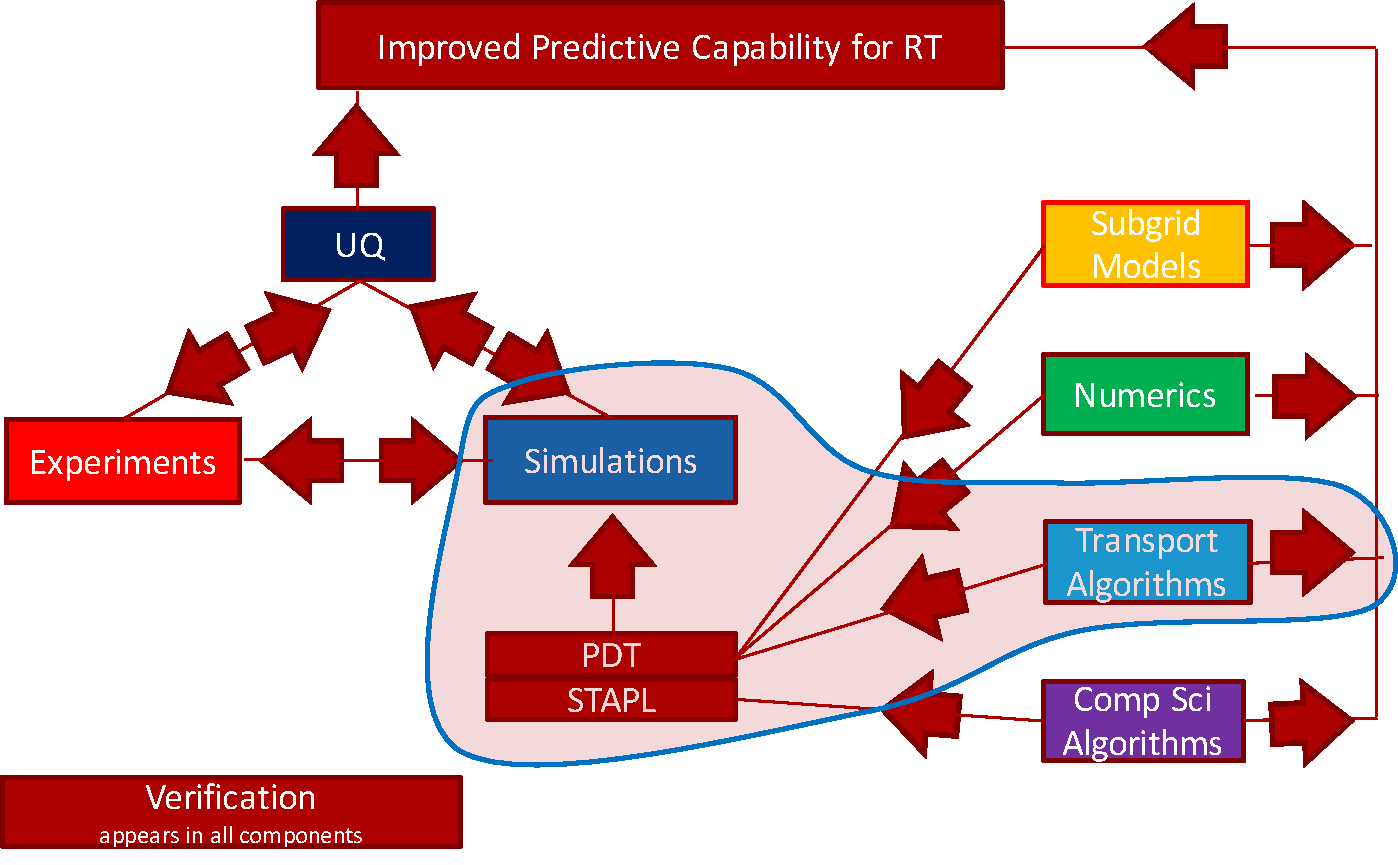
\includegraphics[scale = 0.45 ]{figures/Integration_Slide.pdf}
\end{frame}


\begin{frame}
\tableofcontents
\end{frame}

\section{Introduction}
%\subsection{}
\begin{frame}[t]\frametitle{Motivation}
	\begin{block}{}
	\begin{itemize}
		\item When running any massively parallel code, load balancing is a priority in order to achieve the best possible parallel efficiency.
		\item  A load balanced problem has an equal number of degrees of freedom per processor.
		\item Load balancing a logically Cartesian mesh is ``not difficult", as the user specifies the number of cells being used.
		\item In an unstructured mesh, the user cannot always specify the number of cells they want per processor, and obtaining a load balanced problem is more difficult.
		\item The goal is to implement a load balancing algorithm for unstructured meshes in PDT.
	\end{itemize}
	\end{block}
\end{frame}

\begin{frame}[t]\frametitle{The Triangle Mesh Generator}
	\begin{block}{}
	\begin{itemize}
		\item Unstructured meshes in PDT are generated in 2D using the Triangle Mesh Generator.
		\item These can be extruded to create 3D meshes.
	\end{itemize}	
	\end{block}
	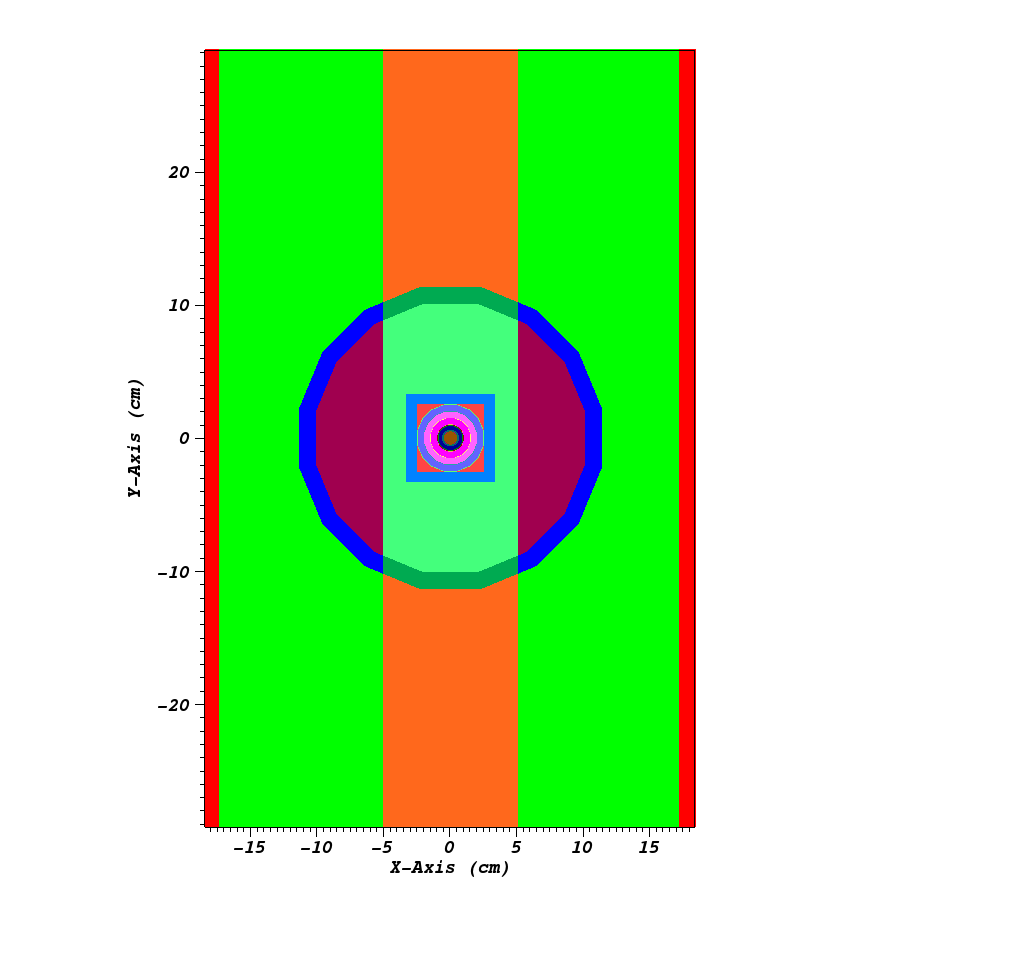
\includegraphics[scale = 0.15]{figures/IM12DPoly.png}
	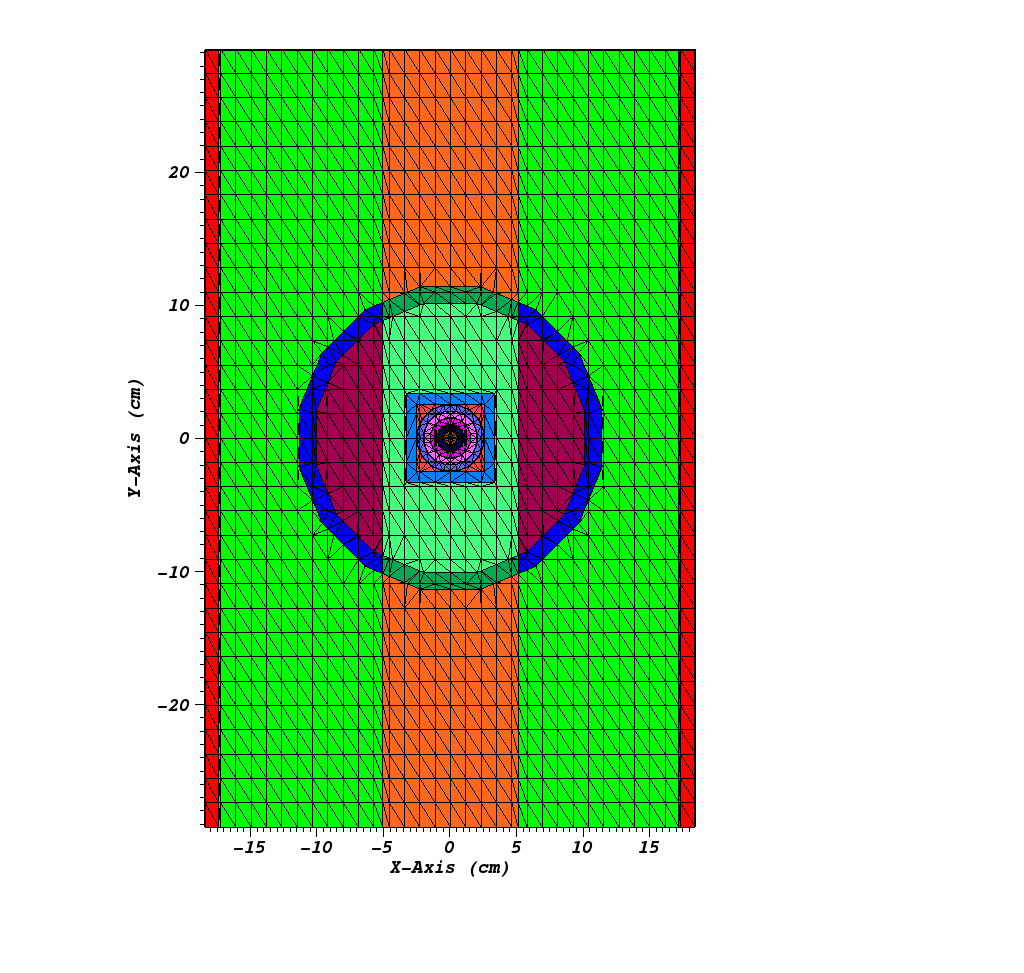
\includegraphics[scale = 0.15]{figures/IM12DMesh.png}
\end{frame}

\section{Load Balance Algorithm}
%\subsection{}

\begin{frame}[t]\frametitle{Partitioning for an Unstructured Mesh}
\begin{block}{}
	\begin{itemize}
	\item The user inputs coordinates for cut lines in the X and Y directions.
	\item The cut lines will determine the number of ``subsets" the problem is partitioned into.
	\item Optimizing the location of these cut lines is the basis of the load balancing algorithm.
	\item A ``subset" is an orthogonal unit that is formed by intersecting cut lines.
	\end{itemize}
\end{block}
\end{frame}

\begin{frame}[t]\frametitle{The Subset}
\centering
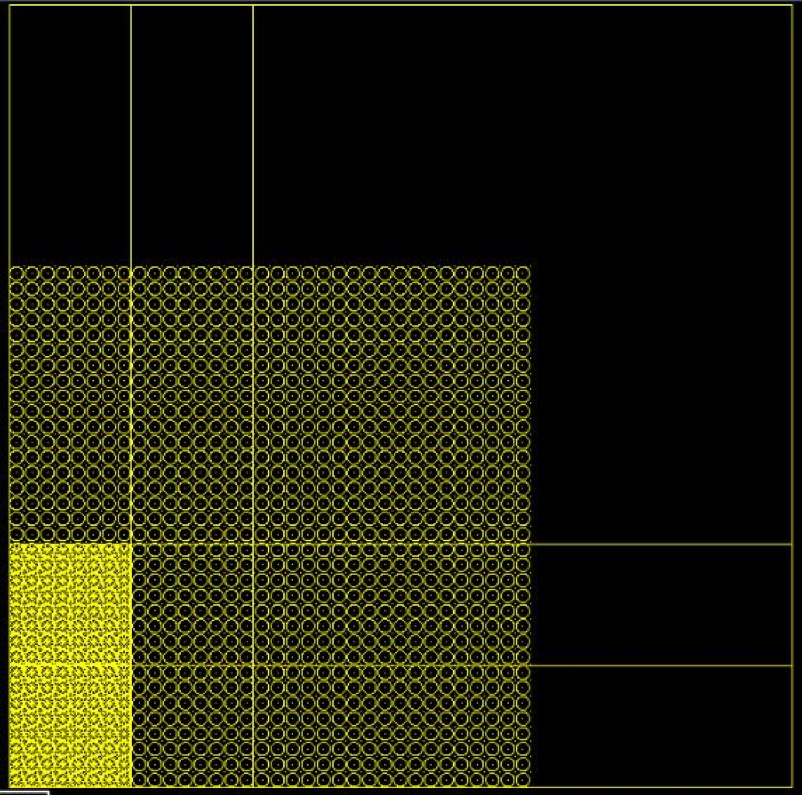
\includegraphics[width = 12 cm, height = 7 cm ]{figures/subsetlattice.png}
\end{frame}

\begin{frame}[t]\frametitle{ Goal and Definitions}
	\begin{block}{}
	
		\begin{itemize}
			\item \textbf{Goal:} Obtain an equal number of cells per processor, which for our purposes means an equal number of cells per subset.
			\item Achieved by optimizing the location of $X_i$ and $Y_j$, the location of the cut lines.
			%\item We define the load balance metric, $f$.
			\item \textbf{Define}:
			\begin{itemize}
			\item $N_{ij}$: The number of cells  in subset ${i,j}$
			%\item Cut Lines: $X_i, Y_j$, $1 <= i <= I-1$, $1 <= j <= J-1$
			\item $f =\frac{\underset{ij}{\text{max}}(N_{ij})}{\frac{N_{tot}}{I\cdot J}}$
			\item $f_I = \underset{i}{\text{max}}[\sum_{j} N_{ij}]/\frac{N_{tot}}{I}$
			\item $f_J = \underset{j}{\text{max}}[\sum_{i} N_{ij}]/\frac{N_{tot}}{J}$
			\end{itemize}
		\end{itemize}
	\end{block}
\end{frame}

\begin{frame}[t]\frametitle{Original Load Balancing Algorithm}
\vspace{-0.5 cm}
\begin{block}{}
\lstinputlisting[language = C++, basicstyle = \footnotesize]{loadbalance.cc}
\end{block}
\end{frame}

\begin{frame}[t]\frametitle{Load Balancing By Dimension Algorithm}
\vspace{-0.5 cm}
\begin{block}{}
\lstinputlisting[language = C++, basicstyle = \footnotesize]{load_balance_by_dimension.cc}
\end{block}
\end{frame}

\begin{frame}[t]\frametitle{Redistribution Function}
\centering
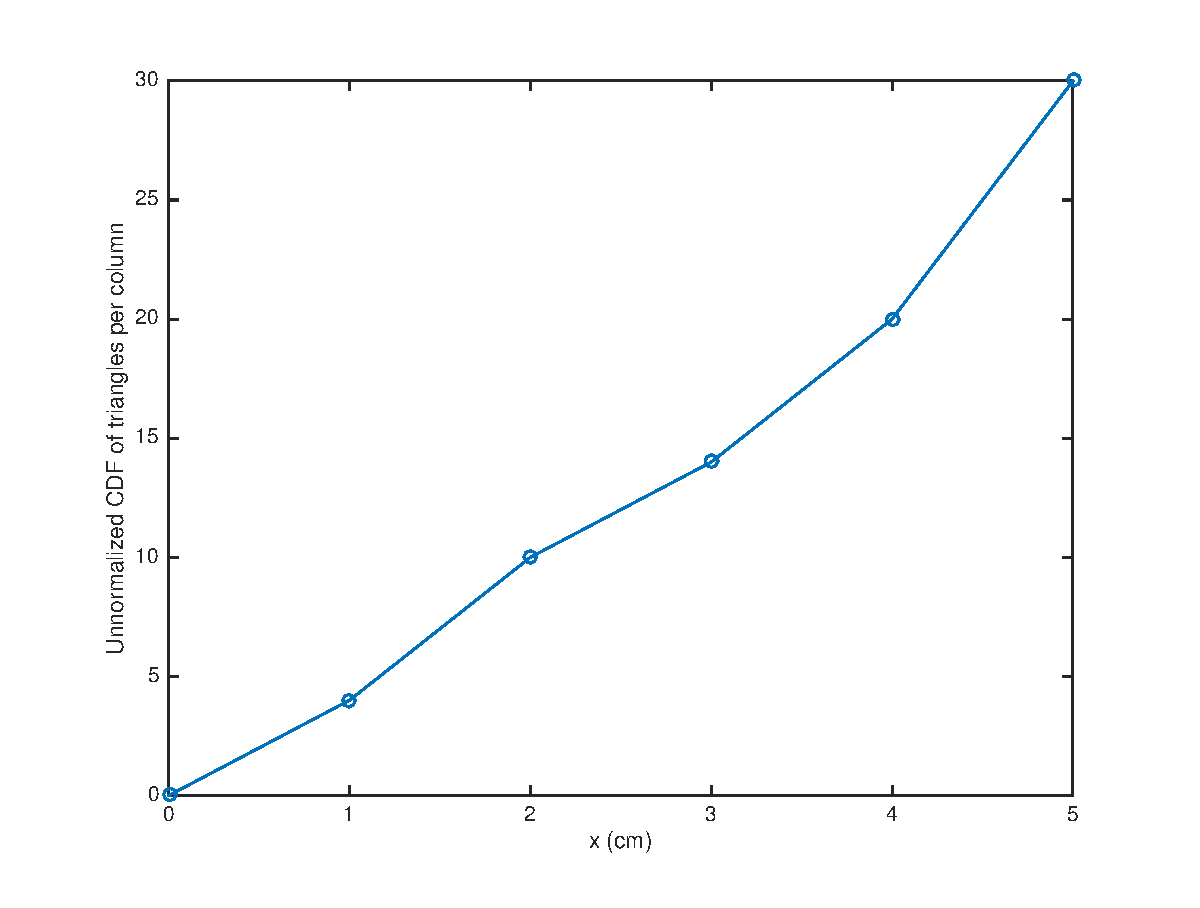
\includegraphics[scale = 0.5]{figures/before_redistribute.eps}
\end{frame}

\begin{frame}[t]\frametitle{Redistribution Function}
\centering
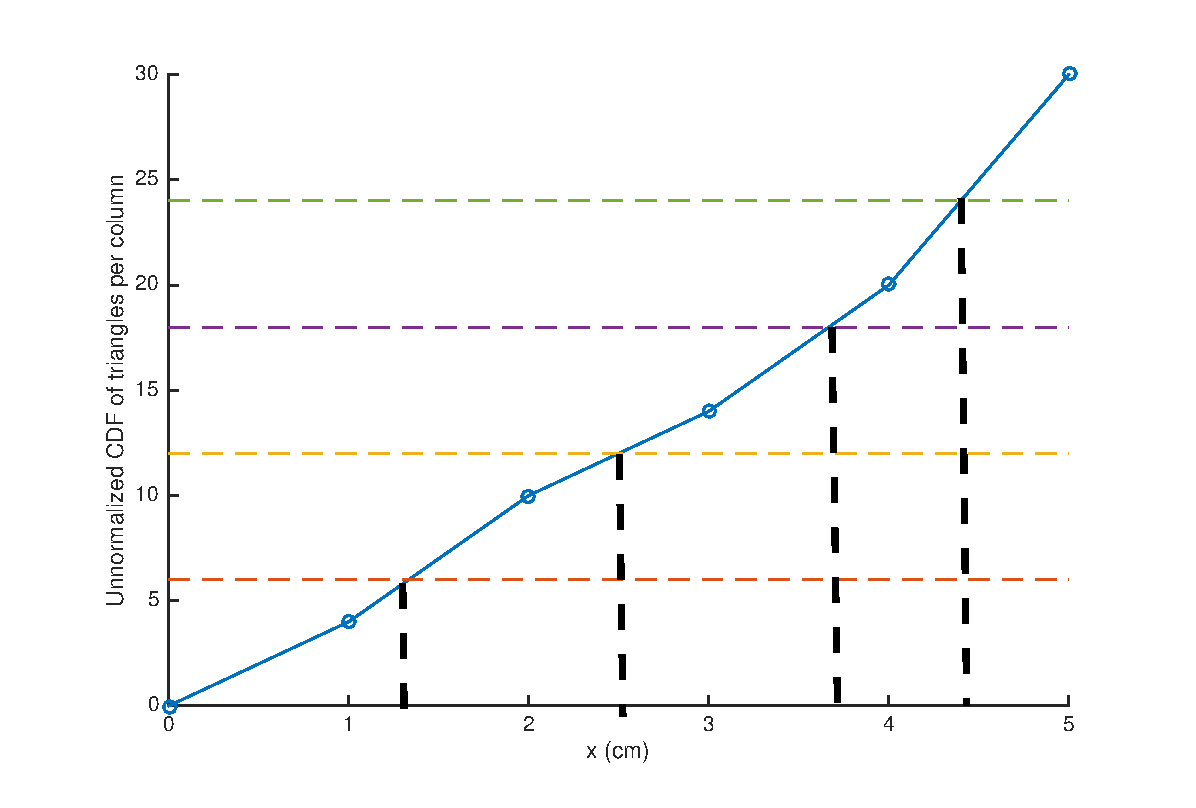
\includegraphics[scale = 0.5]{figures/after_redistribute.eps}
\end{frame}

\section{Load Balancing Results}
%\subsection{}
\begin{frame}[t]\frametitle{Load Balancing Results}
\begin{block}{}
\begin{itemize}
	\item Three test cases were used to study the behavior of the load balancing algorithm.
	\item For each test case, 162 inputs were constructed by varying:
		\begin{itemize}
		\item The number of subsets
		\item The spatial resolution of the mesh (maximum triangle area).
		\end{itemize}
\end{itemize}
\end{block}
\end{frame}

\begin{frame}[t]\frametitle{Test Case 1}
\centering
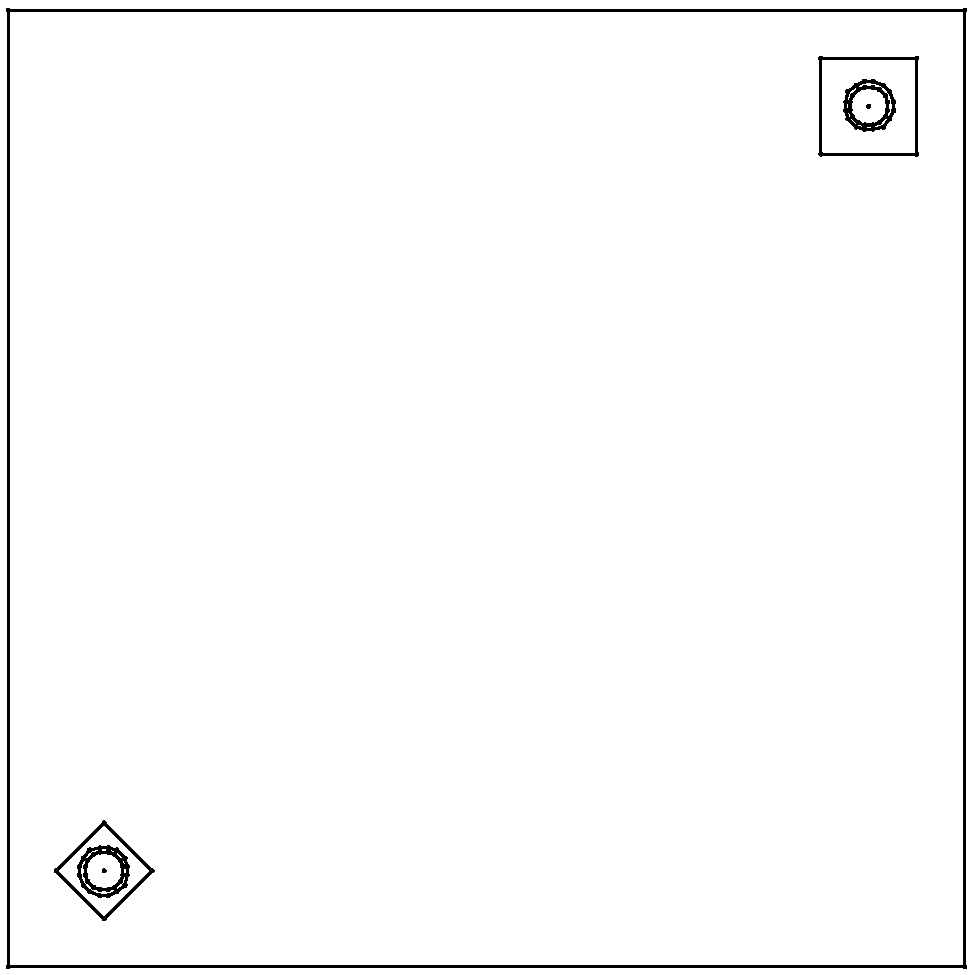
\includegraphics[scale = 0.4]{figures/unbalanced_lattice-eps-converted-to.pdf}
\end{frame}


%Tabulate iterations
\begin{frame}[t]\frametitle{Test Case 1 - Original Load Balancing Method}
\begin{table}[H]
\tiny
\centering
\caption{The best metric behavior of the first test case after \textbf{10 load balancing iterations}.} 
\begin{tabular}{rrrrrrrrrr}
\hline
 Area & N=4 & N=9 & N=16 & N=25 & N=36 & N=49 & N=64 & N=81 & N=100 \\ 
\hline
 Coarse& 1.949 & 1.598 & 3.368 & 2.098 & 2.278 & 2.678 & 2.535 & 2.805 & 3.053 \\
 1.8 &1.458 & 1.940 & 2.449 & 2.590 & 2.980 & 3.441 & 2.957 & 4.657 & 3.434 \\
 1.6 & 1.423 & 1.949 & 2.427 & 2.411 & 3.004 & 3.053 & 3.579 & 4.107 & 4.105 \\
 1.4 & 1.316 & 1.871 & 2.654 & 3.130 & 2.451 & 3.030 & 3.473 & 4.040 & 3.898 \\
 1.2 & 1.298 & 1.765 & 2.462 & 2.656 & 2.592 & 3.178 & 3.144 & 4.282 & \textbf{\cellcolor{blue!25}4.683} \\
 1 & 1.348 & 1.638 & 2.260 & 2.327 & 2.347 & 3.013 & 3.357 & 3.841 & 4.245 \\
 0.8 & 1.257 & 1.513 & 2.017 & 2.792 & 2.018 & 2.617 & 2.884 & 3.423 & 3.629 \\
 0.6 & 1.142 & 1.452 & 1.788 & 2.408 & 2.332 & 2.092 & 2.669 & 2.874 & 3.629 \\
 0.4 & 1.095 & 1.353 & 1.449 & 1.872 & 2.397 & 1.836 & 2.153 & 2.351 & 2.262 \\
 0.2 & 1.046 & 1.136 & 1.336 & 1.545 & 1.648 & 2.049 & 1.678 & 1.790 & 1.714 \\
 0.1 & 1.020 & 1.043 & 1.109 & 1.170 & 1.287 & 1.357 & 1.297 & 1.409 & 1.221 \\
 0.08 & 1.011 & 1.029 & 1.094 & 1.190 & 1.209 & 1.290 & 1.268 & 1.318 & 1.381 \\
 0.06 & 1.005 & 1.031 & 1.037 & 1.105 & 1.087 & 1.189 & 1.177 & 1.283 & 1.068 \\
 0.05 & 1.021 & 1.022 & 1.058 & 1.092 & 1.079 & 1.115 & 1.157 & 1.218 & 1.176 \\
 0.04 & 1.004 & 1.013 & \textbf{\cellcolor{blue!25}1.002} & 1.061 & 1.074 & 1.073 & 1.158 & 1.171 & 1.171 \\
 0.03 & 1.003 & 1.016 & 1.021 & 1.050 & 1.065 & 1.048 & 1.928 & 1.132 & 1.041 \\
 0.02 & 1.004 & 1.008 & 1.010 & 1.034 & 1.024 & 1.028 & 1.574 & 1.075 & 1.094 \\
 0.01& 1.003 & 1.010 & 1.008 & 1.009 & 1.039 & 1.018 & 1.276 & 1.043 & 1.022 \\
\hline
\end{tabular}
\end{table}
\end{frame}

\begin{frame}[t]\frametitle{Test Case 1 - Load Balancing By Dimension}
\begin{table}[H]
\tiny
\centering
\caption{The best metric behavior of the first test case after \textbf{10 load balancing by dimension iterations}.} 
\begin{tabular}{rrrrrrrrrr}
 \hline
 Area & N=4 & N=9 & N=16 & N=25 & N=36 & N=49 & N=64 & N=81 & N=100 \\ 
\hline
 Coarse & 1.854 & 1.205 & 1.475 & 1.398 & 1.260 & 1.367 & 1.428 & 1.625 & 1.639 \\
  1.800 & 1.079 & 1.392 & 1.523 & 1.722 & 2.036 & 2.315 & 2.421 & 3.962 & 3.587 \\
  1.600 & 1.044 & 1.704 & 1.536 & 1.566 & 1.791 & 2.126 & 2.492 & 3.417 & 3.807 \\
  1.400 & 1.073 & 1.152 & 1.509 & 1.756 & 1.811 & 2.183 & 2.475 & 2.911 & \textbf{\cellcolor{blue!25}3.974} \\
  1.200 & 1.037 & 1.125 & 1.515 & 1.718 & 1.972 & 2.611 & 2.628 & 3.816 & 3.205 \\
  1.000 & 1.047 & 1.209 & 1.180 & 1.763 & 1.494 & 1.928 & 2.564 & 3.744 & 3.953 \\
  0.800 & 1.077 & 1.193 & 1.246 & 1.343 & 1.417 & 2.949 & 2.411 & 3.560 & 3.629 \\
  0.600 & 1.066 & 1.112 & 1.388 & 1.455 & 1.521 & 1.837 & 1.769 & 2.586 & 3.381 \\
  0.400 & 1.095 & 1.032 & 1.145 & 1.221 & 1.479 & 1.355 & 1.554 & 2.038 & 1.838 \\
  0.200 & 1.046 & 1.049 & 1.075 & 1.149 & 1.173 & 1.174 & 1.210 & 1.251 & 1.571 \\
  0.100 & 1.020 & 1.043 & 1.023 & 1.071 & 1.103 & 1.138 & 1.129 & 1.091 & 1.205 \\
  0.080 & 1.011 & 1.029 & 1.094 & 1.072 & 1.076 & 1.097 & 1.068 & 1.071 & 1.213 \\
  0.060 & 1.005 & 1.031 & 1.037 & 1.016 & 1.087 & 1.096 & 1.093 & 1.095 & 1.068 \\
  0.050 & 1.021 & 1.022 & 1.058 & 1.092 & 1.079 & 1.062 & 1.090 & 1.075 & 1.088 \\
  0.040 & 1.004 & 1.013 & 1\textbf{\cellcolor{blue!25}.002} & 1.061 & 1.074 & 1.073 & 1.067 & 1.090 & 1.100 \\
  0.030 & 1.003 & 1.016 & 1.021 & 1.050 & 1.065 & 1.048 & 1.038 & 1.061 & 1.041 \\
  0.020 & 1.004 & 1.008 & 1.010 & 1.034 & 1.024 & 1.028 & 1.058 & 1.075 & 1.094 \\
  0.010 & 1.003 & 1.010 & 1.008 & 1.009 & 1.039 & 1.018 & 1.054 & 1.043 & 1.022 \\
\hline
\end{tabular}
\end{table}
\end{frame}

%Table Diff
\begin{frame}\frametitle{Test Case 1 - Improvement}
\begin{table}[H]
\tiny
\centering
\caption{The improvement with the load balancing by dimension method.} 
\begin{tabular}{rrrrrrrrrr}
 \hline
 Area & N=4 & N=9 & N=16 & N=25 & N=36 & N=49 & N=64 & N=81 & N=100 \\ 
\hline
 Coarse & 0.049 & 0.246 & \textbf{\cellcolor{blue!25}0.562} & 0.334 & 0.447 &  0.489 & 0.437 &  0.421 &  0.463 \\
  1.800 & 0.260 & 0.282 & 0.378 & 0.335 & 0.317 &  0.327 & 0.181 &  0.149 & -0.045 \\
  1.600 & 0.266 & 0.126 & 0.367 & 0.350 & 0.404 &  0.304 & 0.304 &  0.168 &  0.072 \\
  1.400 & 0.185 & 0.384 & 0.431 & 0.439 & 0.261 &  0.279 & 0.287 &  0.279 & -0.020 \\
  1.200 & 0.201 & 0.363 & 0.384 & 0.353 & 0.239 &  0.178 & 0.164 &  0.109 &  0.316 \\
  1.000 & 0.223 & 0.262 & 0.478 & 0.242 & 0.364 &  0.360 & 0.236 &  0.025 &  0.069 \\
  0.800 & 0.143 & 0.211 & 0.382 & 0.519 & 0.298 & \textbf{\cellcolor{blue!25}-0.127} & 0.164 & -0.040 &  0.000 \\
  0.600 & 0.067 & 0.234 & 0.224 & 0.396 & 0.347 &  0.122 & 0.337 &  0.100 &  0.068 \\
  0.400 & 0.000 & 0.237 & 0.210 & 0.347 & 0.383 &  0.262 & 0.278 &  0.133 &  0.188 \\
  0.200 & 0.000 & 0.076 & 0.196 & 0.256 & 0.288 &  0.427 & 0.279 &  0.301 &  0.083 \\
  0.100 & 0.000 & 0.000 & 0.078 & 0.085 & 0.143 &  0.161 & 0.130 &  0.226 &  0.013 \\
  0.080 & 0.000 & 0.000 & 0.000 & 0.099 & 0.110 &  0.150 & 0.158 &  0.188 &  0.122 \\
  0.060 & 0.000 & 0.000 & 0.000 & 0.080 & 0.000 &  0.078 & 0.071 &  0.147 &  0.000 \\
  0.050 & 0.000 & 0.000 & 0.000 & 0.000 & 0.000 &  0.048 & 0.058 &  0.117 &  0.075 \\
  0.040 & 0.000 & 0.000 & 0.000 & 0.000 & 0.000 &  0.000 & 0.079 &  0.069 &  0.061 \\
  0.030 & 0.000 & 0.000 & 0.000 & 0.000 & 0.000 &  0.000 & 0.462 &  0.062 &  0.000 \\
  0.020 & 0.000 & 0.000 & 0.000 & 0.000 & 0.000 &  0.000 & 0.328 &  0.000 &  0.000 \\
  0.010 & 0.000 & 0.000 & 0.000 & 0.000 & 0.000 &  0.000 & 0.174 &  0.000 &  0.000 \\
\hline
\end{tabular}
\end{table}
\end{frame}

\begin{frame}[t]\frametitle{Test Case 2}
\centering
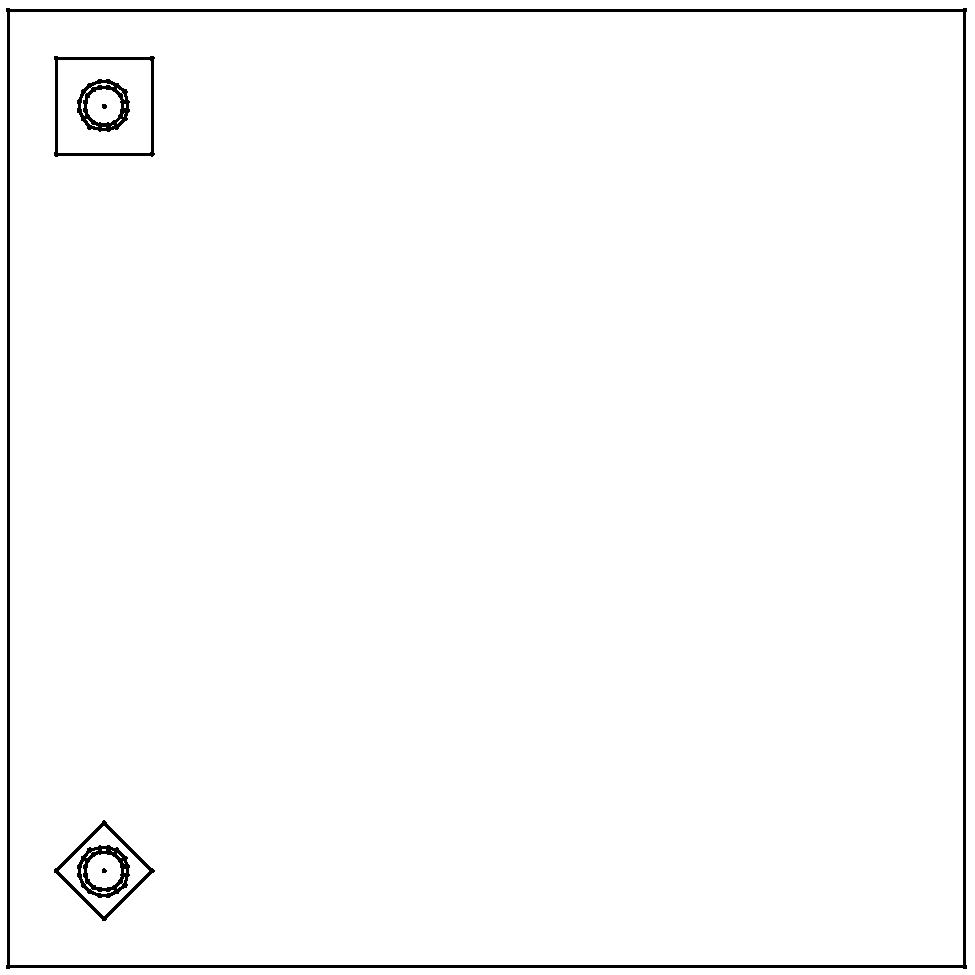
\includegraphics[scale = 0.4]{figures/unbalanced_pins_same_side-eps-converted-to.pdf}
\end{frame}


\begin{frame}[t]\frametitle{Test Case 2 - Original Load Balancing Method}
\begin{table}[H]
\centering
\tiny
\caption{The best metric behavior of the second test case after \textbf{10 load balancing iterations}.} 
\begin{tabular}{rrrrrrrrrr}
 \hline
 Area & N=4 & N=9 & N=16 & N=25 & N=36 & N=49 & N=64 & N=81 & N=100 \\ 
\hline
 Coarse & 1.854 & 1.361 & 1.765 & 1.479 & 1.742 & 1.595 & 1.792 & 1.820 & 1.923 \\
  1.800 & 1.176 & 1.336 & 1.882 & 2.375 & 2.269 & 2.359 & 2.544 & 3.841 & \textbf{\cellcolor{blue!25}4.874} \\
  1.600 & 1.109 & 1.482 & 1.783 & 1.701 & 1.990 & 2.421 & 2.848 & 3.345 & 2.989 \\
  1.400 & 1.133 & 1.366 & 1.854 & 1.746 & 1.882 & 2.600 & 2.833 & 3.617 & 2.692 \\
  1.200 & 1.153 & 1.506 & 1.575 & 1.599 & 2.162 & 2.270 & 2.562 & 3.355 & 3.771 \\
  1.000 & 1.132 & 1.418 & 1.729 & 1.694 & 1.581 & 2.452 & 2.491 & 3.231 & 3.902 \\
  0.800 & 1.139 & 1.355 & 1.437 & 1.610 & 1.940 & 2.167 & 2.152 & 2.250 & 2.936 \\
  0.600 & 1.053 & 1.360 & 1.604 & 1.705 & 1.687 & 1.960 & 1.902 & 2.458 & 2.500 \\
  0.400 & 1.095 & 1.176 & 1.401 & 1.534 & 1.771 & 1.797 & 1.841 & 1.792 & 2.262 \\
  0.200 & 1.043 & 1.140 & 1.183 & 1.364 & 1.561 & 1.741 & 1.587 & 1.495 & 1.714 \\
  0.100 & 1.028 & 1.042 & 1.114 & 1.193 & 1.284 & 1.335 & 1.268 & 1.227 & 1.283 \\
  0.080 & 1.013 & 1.037 & 1.091 & 1.190 & 1.210 & 1.293 & 1.197 & 1.236 & 1.178 \\
  0.060 & 1.007 & 1.033 & 1.037 & 1.105 & 1.087 & 1.205 & 1.183 & 1.281 & 1.101 \\
  0.050 & 1.021 & 1.026 & 1.050 & 1.088 & 1.061 & 1.115 & 1.182 & 1.215 & 1.176 \\
  0.040 & 1.005 & 1.019 & \textbf{\cellcolor{blue!25}1.001} & 1.061 & 1.075 & 1.073 & 1.098 & 1.173 & 1.171 \\
  0.030 & 1.005 & 1.013 & 1.021 & 1.045 & 1.060 & 1.050 & 1.265 & 1.101 & 1.041 \\
  0.020 & 1.006 & 1.017 & 1.008 & 1.034 & 1.022 & 1.024 & 1.186 & 1.076 & 1.097 \\
  0.010 & 1.003 & 1.010 & 1.008 & 1.009 & 1.039 & 1.018 & 1.276 & 1.043 & 1.022 \\
\hline
\end{tabular}
\end{table}
\end{frame}

\begin{frame}[t]\frametitle{Test Case 2 - Load Balancing By Dimension}
\begin{table}[H]
\tiny
\centering
\caption{The best metric behavior of the second test case after \textbf{10 load balancing by dimension iterations}.} 
\begin{tabular}{rrrrrrrrrr}
 \hline
 Area & N=4 & N=9 & N=16 & N=25 & N=36 & N=49 & N=64 & N=81 & N=100 \\ 
\hline
 Coarse & 1.854 & 1.134 & 1.672 & 1.324 & 1.653 & 1.518 & 1.542 & 1.401 & 1.520 \\
  1.800 & 1.099 & 1.135 & 1.438 & 1.868 & 1.753 & 1.840 & 2.740 & 3.262 & 1.690 \\
  1.600 & 1.086 & 1.118 & 1.598 & 1.558 & 1.802 & 2.350 & \textbf{\cellcolor{blue!25}4.700} & 3.776 & 3.441 \\
  1.400 & 1.052 & 1.101 & 1.432 & 1.768 & 1.966 & 2.000 & 2.688 & 2.827 & 3.169 \\
  1.200 & 1.042 & 1.183 & 1.419 & 1.542 & 1.620 & 2.192 & 3.939 & 3.237 & 3.111 \\
  1.000 & 1.057 & 1.207 & 1.315 & 1.331 & 1.453 & 1.698 & 2.436 & 2.455 & 3.524 \\
  0.800 & 1.051 & 1.097 & 1.204 & 1.570 & 1.510 & 1.753 & 1.738 & 2.232 & 2.576 \\
  0.600 & 1.053 & 1.091 & 1.070 & 1.215 & 1.424 & 1.765 & 1.613 & 1.678 & 2.456 \\
  0.400 & 1.095 & 1.087 & 1.120 & 1.212 & 1.226 & 1.346 & 1.215 & 2.078 & 2.128 \\
  0.200 & 1.043 & 1.038 & 1.074 & 1.112 & 1.238 & 1.082 & 1.311 & 1.564 & 1.522 \\
  0.100 & 1.028 & 1.042 & 1.097 & 1.042 & 1.098 & 1.124 & 1.129 & 1.095 & 1.204 \\
  0.080 & 1.013 & 1.037 & 1.091 & 1.085 & 1.090 & 1.128 & 1.092 & 1.110 & 1.178 \\
  0.060 & 1.007 & 1.033 & 1.037 & 1.014 & 1.087 & 1.082 & 1.048 & 1.092 & 1.034 \\
  0.050 & 1.021 & 1.026 & 1.050 & 1.088 & 1.061 & 1.052 & 1.083 & 1.079 & 1.075 \\
  0.040 & 1.005 & 1.019 & \textbf{\cellcolor{blue!25}1.001} & 1.061 & 1.075 & 1.073 & 1.081 & 1.093 & 1.145 \\
  0.030 & 1.005 & 1.013 & 1.021 & 1.045 & 1.060 & 1.050 & 1.061 & 1.076 & 1.041 \\
  0.020 & 1.006 & 1.017 & 1.008 & 1.034 & 1.022 & 1.024 & 1.095 & 1.076 & 1.097 \\
  0.010 & 1.003 & 1.010 & 1.008 & 1.009 & 1.039 & 1.018 & 1.092 & 1.043 & 1.022 \\
\hline
\end{tabular}
\end{table}
\end{frame}

%Test Case 2 Improvement
\begin{frame}[t]\frametitle{Test Case 2 - Improvement}
\begin{table}[H]
\centering
\tiny
\caption{The improvement with the load balancing by dimension method.} 
\begin{tabular}{rrrrrrrrrr}
 \hline
 Area & N=4 & N=9 & N=16 & N=25 & N=36 & N=49 & N=64 & N=81 & N=100 \\ 
\hline
 Coarse & 0.000 & 0.167 & 0.053 &  0.105 &  0.051 & 0.049 &  0.139 &  0.230 &  0.210 \\
  1.800 & 0.066 & 0.151 & 0.236 &  0.214 &  0.228 & 0.220 & -0.077 &  0.151 &  \textbf{\cellcolor{blue!25}0.653} \\
  1.600 & 0.021 & 0.246 & 0.104 &  0.084 &  0.094 & 0.030 & \textbf{\cellcolor{blue!25}-0.650} & -0.129 & -0.151 \\
  1.400 & 0.072 & 0.193 & 0.227 & -0.012 & -0.045 & 0.231 &  0.051 &  0.218 & -0.177 \\
  1.200 & 0.096 & 0.215 & 0.099 &  0.036 &  0.251 & 0.035 & -0.537 &  0.035 &  0.175 \\
  1.000 & 0.066 & 0.149 & 0.239 &  0.214 &  0.081 & 0.308 &  0.022 &  0.240 &  0.097 \\
  0.800 & 0.078 & 0.191 & 0.162 &  0.025 &  0.221 & 0.191 &  0.192 &  0.008 &  0.123 \\
  0.600 & 0.000 & 0.198 & 0.333 &  0.288 &  0.156 & 0.099 &  0.152 &  0.318 &  0.018 \\
  0.400 & 0.000 & 0.075 & 0.201 &  0.210 &  0.308 & 0.251 &  0.340 & -0.159 &  0.060 \\
  0.200 & 0.000 & 0.089 & 0.092 &  0.185 &  0.207 & 0.379 &  0.174 & -0.046 &  0.112 \\
  0.100 & 0.000 & 0.000 & 0.015 &  0.126 &  0.145 & 0.158 &  0.109 &  0.108 &  0.062 \\
  0.080 & 0.000 & 0.000 & 0.000 &  0.089 &  0.099 & 0.128 &  0.088 &  0.102 &  0.000 \\
  0.060 & 0.000 & 0.000 & 0.000 &  0.082 &  0.000 & 0.102 &  0.115 &  0.148 &  0.061 \\
  0.050 & 0.000 & 0.000 & 0.000 &  0.000 &  0.000 & 0.057 &  0.084 &  0.112 &  0.086 \\
  0.040 & 0.000 & 0.000 & 0.000 &  0.000 &  0.000 & 0.000 &  0.016 &  0.069 &  0.022 \\
  0.030 & 0.000 & 0.000 & 0.000 &  0.000 &  0.000 & 0.000 &  0.162 &  0.022 &  0.000 \\
  0.020 & 0.000 & 0.000 & 0.000 &  0.000 &  0.000 & 0.000 &  0.077 &  0.000 &  0.000 \\
  0.010 & 0.000 & 0.000 & 0.000 &  0.000 &  0.000 & 0.000 &  0.144 &  0.000 &  0.000 \\
\hline
\end{tabular}
\end{table}
\end{frame}

\begin{frame}[t]\frametitle{IM1}
\centering
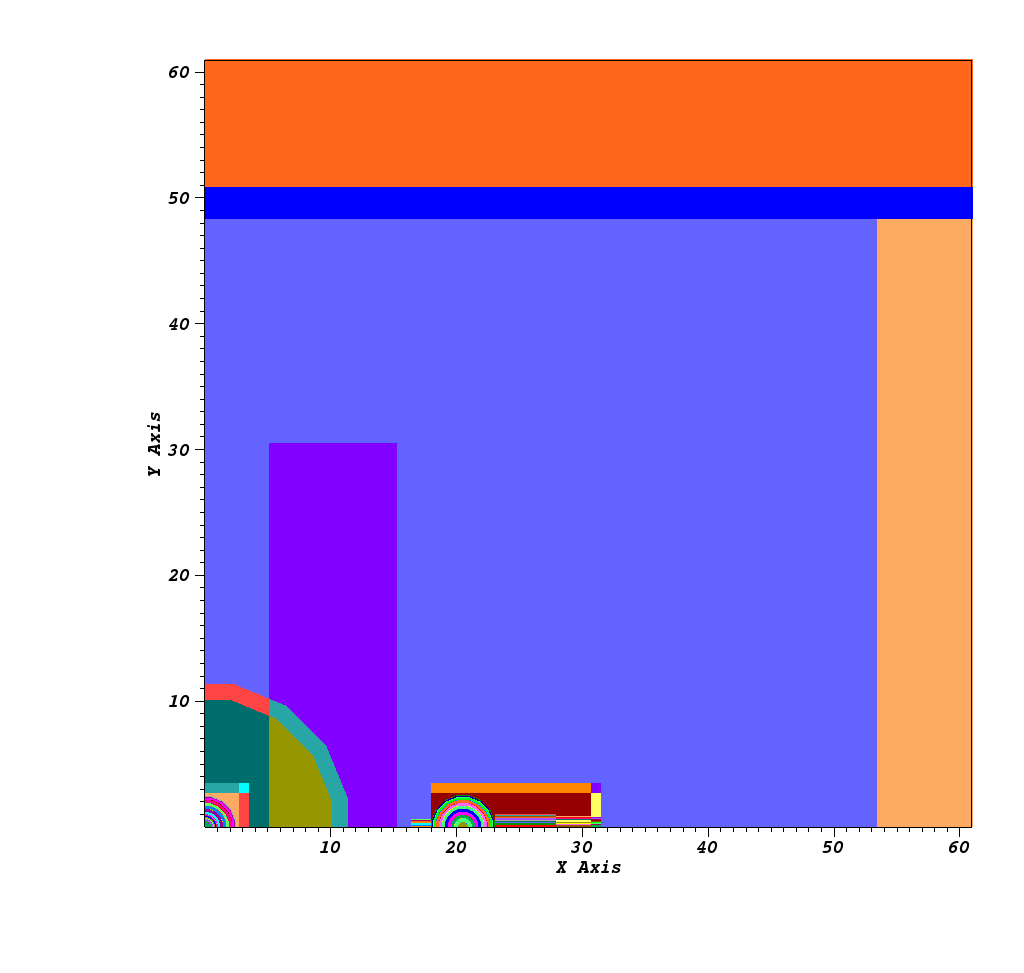
\includegraphics[scale=0.25]{figures/IM12D_val.png}
\end{frame}

\begin{frame}[t]\frametitle{IM1 - Original Load Balancing, f = 2.63}
\centering
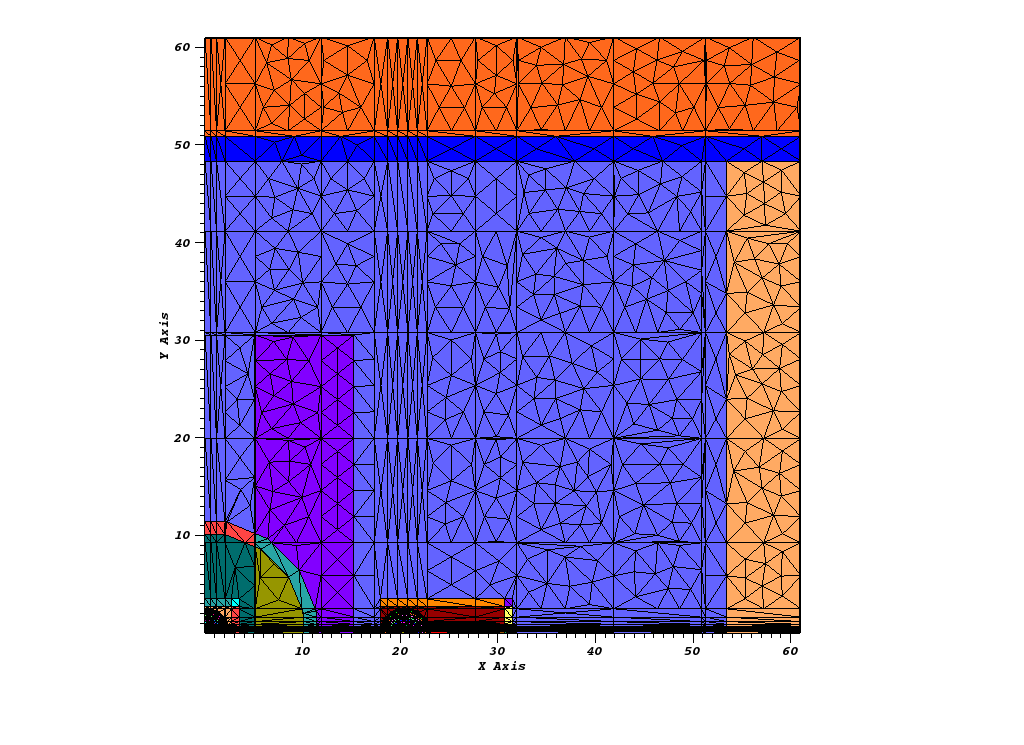
\includegraphics[scale=0.33]{figures/IM1_old_load_balance.png}
\end{frame}

\begin{frame}[t]\frametitle{IM1 - Load Balancing By Dimension, f = 1.76}
\centering
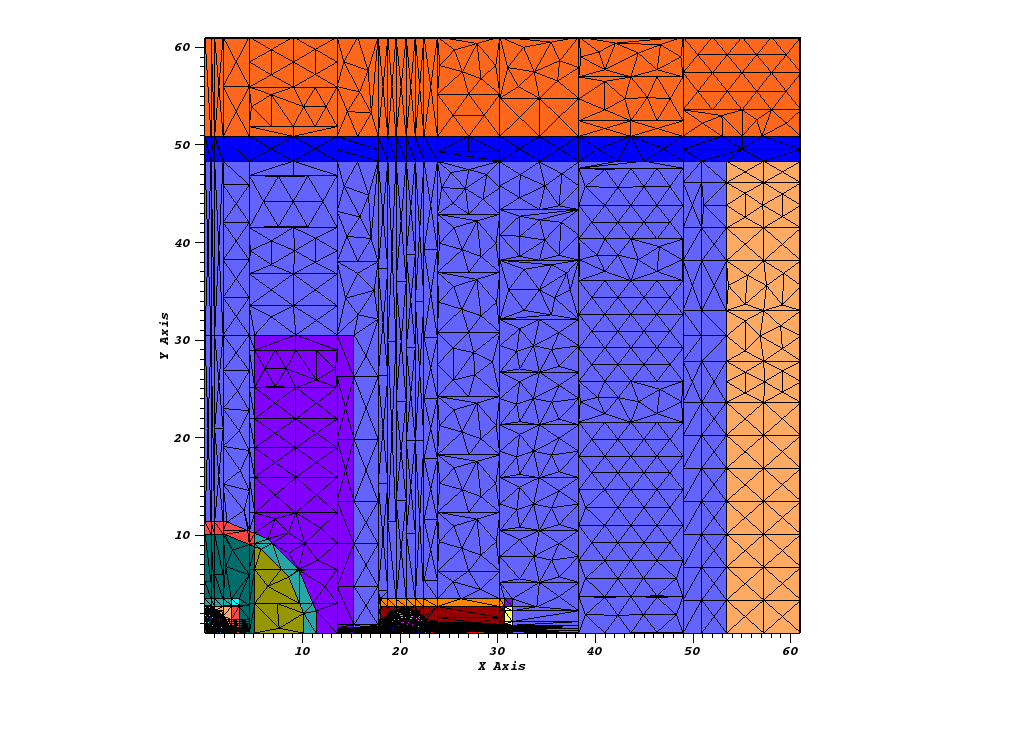
\includegraphics[scale=0.33]{figures/IM1_new_load_balance.png}
\end{frame}

\section{Conclusions}
%\subsection{}
\begin{frame}[t]\frametitle{Conclusions}
\begin{block}{}
\begin{itemize}
\item The effectiveness of the load balancing algorithm depends on the spatial distribution of fine geometric features, the maximum triangle area used, and the number of subsets the domain is decomposed into.
\item Good improvement is seen for Test Cases 1 and 2, and especially the IM1 problem.m
\item More tinkering with the load balancing by dimension algorithm will be done to study its behavior and potential improvements.
\end{itemize}
\end{block}
\end{frame}

\begin{frame}[t]\frametitle{Future Work - Meshing}
\begin{block}{}
\begin{itemize}
\item Moving away from the Triangle Mesh Generator
	\begin{itemize}
		\item Lack of support
		\item Unable to enforce mesh quality consistently while load balancing problems
	\end{itemize}
\item Current path forward involves a collaborative effort with Richard Vega (TAMU/Sandia) using a combination of Cubit and OpenFoam.
	\begin{itemize}
		\item Splitting the mesh into subsets rather than the problem geometry
	\end{itemize}
\end{itemize}
\end{block}
\end{frame}

\begin{frame}[t]\frametitle{Future Work - Load Balancing}
\begin{block}{}
\begin{itemize}
\item Two more paths for improving the load balancing algorithm have been outlined.
\begin{itemize} 
\item Adaptively splitting the subsets that have large cell counts into smaller subsets, and redistributing subsets amongst processors.
\item Taking advantage of nested parallelism to assign more parallel processes at subsets that require more work to be done.
\end{itemize}
\item Studying the behavior of the communication penalty while load balancing (brought up by Derek Gaston at M\&C 2017).
\end{itemize}
\end{block}
\end{frame}

\begin{frame}[t]\frametitle{Initial Setup}
\centering
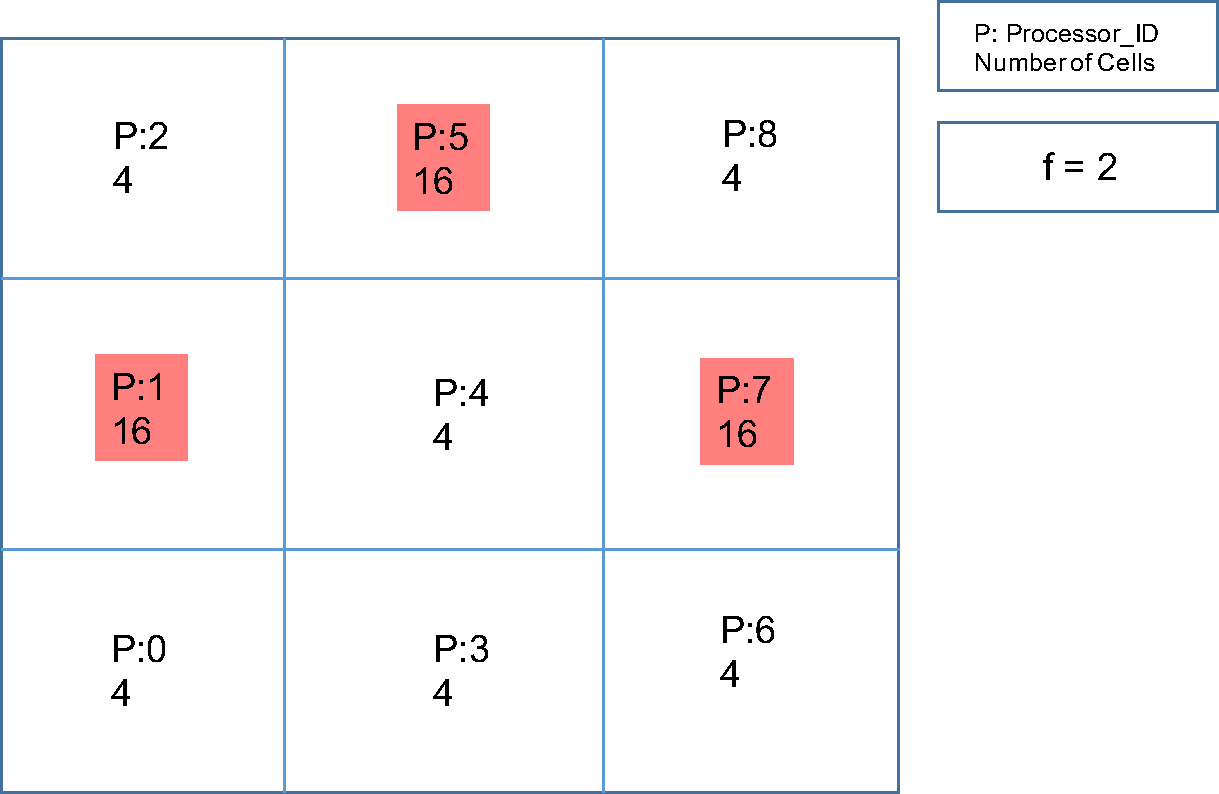
\includegraphics[scale=0.5]{figures/initial_setup.pdf}
\end{frame}

\begin{frame}[t]\frametitle{Adaptively Refine Subsets}
\centering
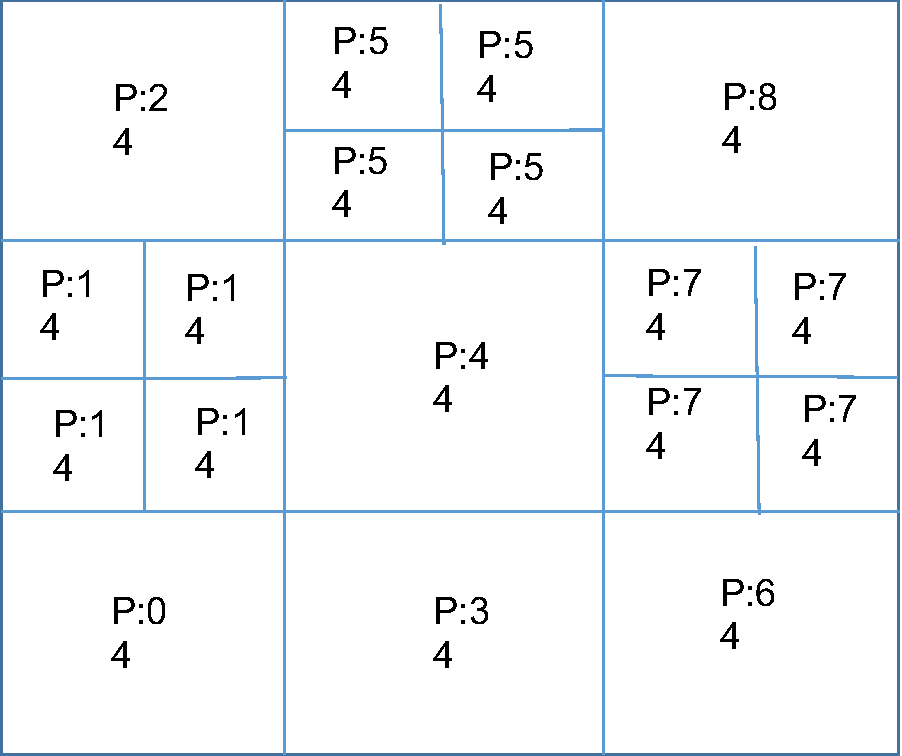
\includegraphics[scale=0.5]{figures/amr.pdf}
\end{frame}

\begin{frame}[t]\frametitle{Subset Redistribution}
\begin{minipage}{0.15\textwidth}
\begin{footnotesize}
$f = 1$
\end{footnotesize}
\end{minipage}
\begin{minipage}{0.8\textwidth}
\centering
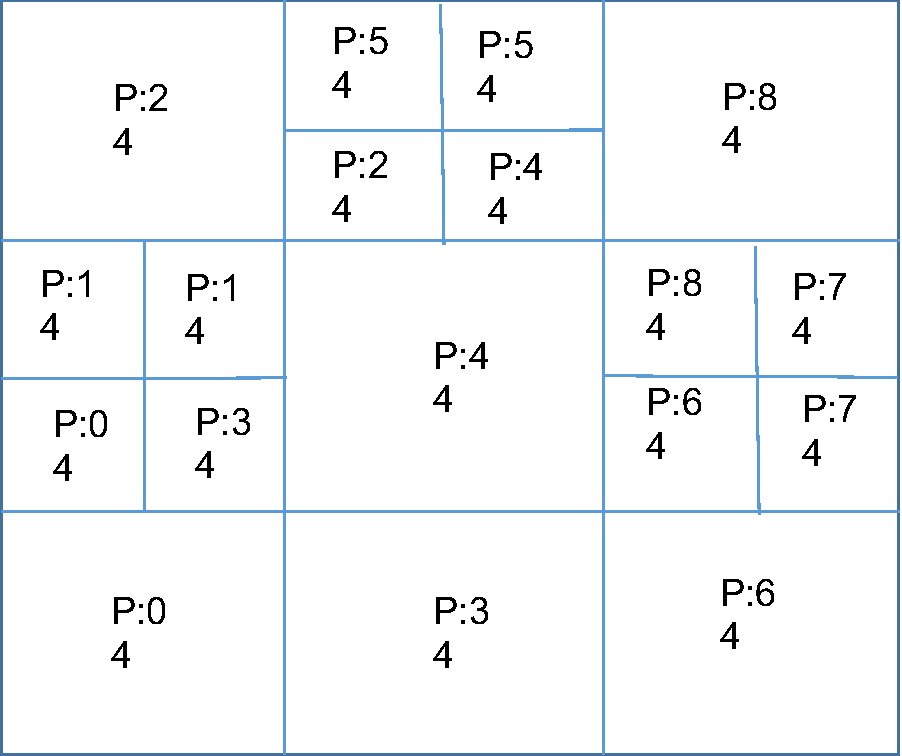
\includegraphics[scale=0.5]{figures/domain_overloading.pdf}
\end{minipage}
\end{frame}

\begin{frame}[t]\frametitle{Nested Parallelism}
\centering
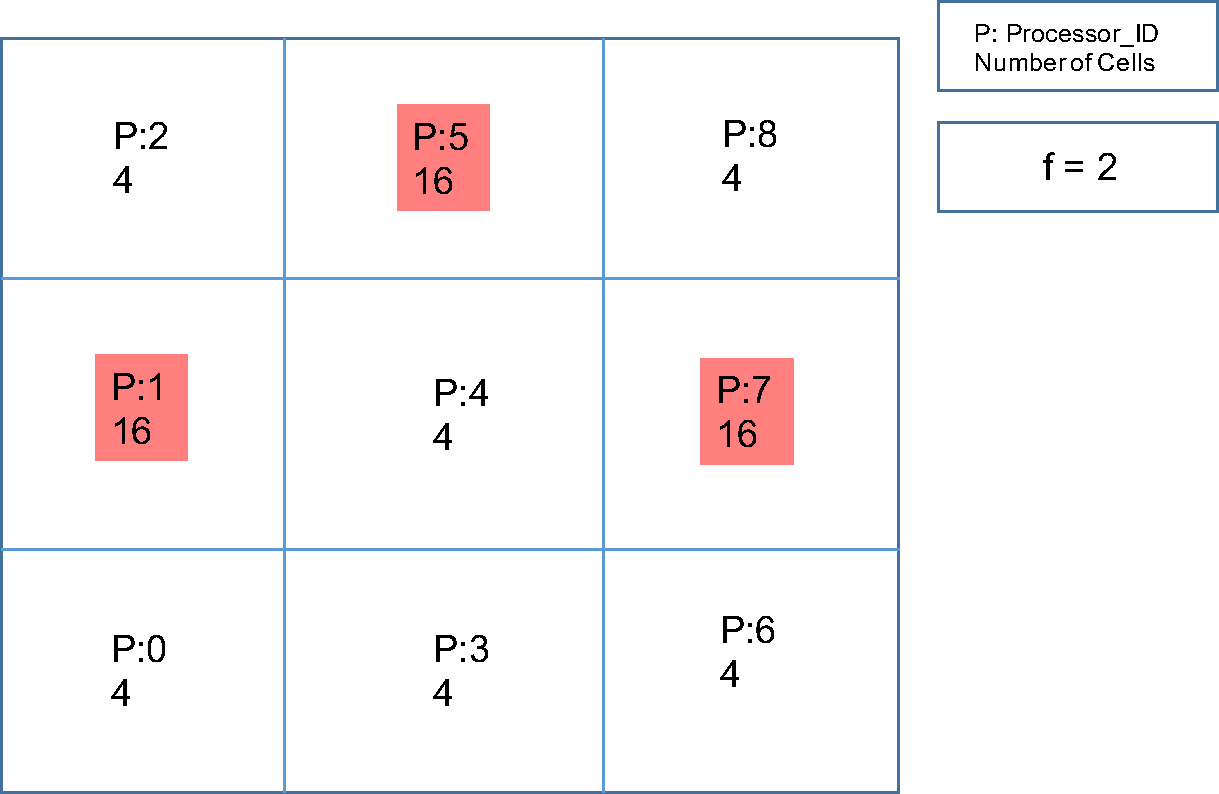
\includegraphics[scale=0.5]{figures/initial_setup.pdf}
\end{frame}

\begin{frame}[t]\frametitle{Acknowledgements}
\begin{block}{}
A special thank you to the following individuals for their help and support:
\begin{itemize}
\item Drs. Ragusa, Morel, Adams, and Popov
\item Michael Adams, Daryl Hawkins, and Dr. Timmie Smith
\item Dr. Andrew Till
\item The CERT team and fellow grad students
\item PSAAP-II 
\end{itemize}
\end{block}
\end{frame}

%\begin{frame}[allowframebreaks]{Bibliography}
%\bibliographystyle{alpha}
%\bibliography{science}
% \nocite{*}
%\end{frame}



%\section{\ }
%\begin{frame}[t]\frametitle{Sources}
%	\nocite{Dubcova20111182}
%	\nocite{CHAUVET}
%	\bibliographystyle{ieeetr}
%	\bibliography{science.bib}
%	
%	
%\end{frame}
%



\end{document}